\section{Body - defining Bodies}

An INI file can contain an arbitrary number of sections defining bodies. Each body section is opened by \lstinline{[BODY: NAME]} where \lstinline{BODY:} defines the bodies type and \lstinline{NAME} is an unique name to tell different bodies with equal types apart. The \lstinline{order} and the \lstinline{shift_vector} parameters are supported by all bodies but mandatory. They will be explained later (???TODO ADD REFERENCE???).

\paragraph{Important:} All vectors inside a body section are specified in lattice coordinates by default. For every vector specified in cartesian coordinates the additional parameter \lstinline{someparameter_coordsys} must be added. Its value is either \lstinline{lattice} or \lstinline{cartesian}.

\subsection{Non-periodic bodies}
\subsubsection{Sphere}
The simplest body one can specify is a sphere. The body's section is opened by \lstinline{[sphere: NAME]}. Its size is determined by a  vector pointing from the center of the sphere (at the origin of the coordinate system) to an arbitrary point on its surface.

\paragraph{Parameters}
\begin{description}
 \item{\lstinline{radius_vector}} Vector whose length specifies the radius of the sphere.
\end{description}

\paragraph{Example}\ 

\lstinputlisting{srcexamples/sphere.ini}
\ \\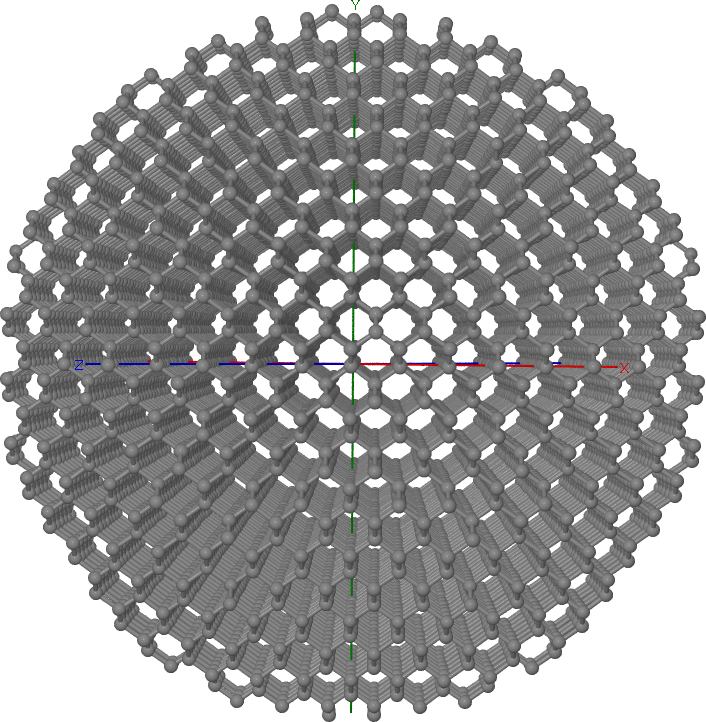
\includegraphics[width=0.6\textwidth]{srcexamples/sphere.png}
\subsection{1D-periodic bodies}
\subsection{2D-periodic bodies}
